% This file provides an example Beamer presentation using the RWTH theme
% showcasing some of the more common options, similar to the Powerpoint version
% 12.11.2014: Revision 1 (Harold Bruintjes, Tim Lange)
% 23.10.2015: Edit by Kai Frantzen

% For RWTH, beamer should be loaded with class option t (top)
\documentclass[t]{beamer}
\usepackage[utf8]{inputenc}
\usepackage{amssymb}
\usepackage{pifont}
\usepackage{multirow}
\usepackage{booktabs}
\usepackage{adjustbox} 
 
% German style date formatting (footer)
\usepackage[ddmmyyyy]{datetime}
\renewcommand{\dateseparator}{.}

% Format the captions used for figures etc.
\usepackage[compatibility=false]{caption}
\captionsetup{singlelinecheck=off,justification=raggedleft,labelformat=empty,labelsep=none}

% regular 4:3 theme for i6 internal usage
\usetheme{rwth}
% uncomment if you want to use 16:9 format
% \usetheme[wide]{rwth}

\graphicspath{{figures/}}

% https://tex.stackexchange.com/questions/426088/texlive-pretest-2018-beamer-and-subfig-collide
\makeatletter
\let\@@magyar@captionfix\relax
\makeatother

% https://tex.stackexchange.com/questions/83440/inputenc-error-unicode-char-u8-not-set-up-for-use-with-latex
% https://gist.github.com/beniwohli/798549
%\DeclareUnicodeCharacter{25A0}{\ding{110}}
\DeclareUnicodeCharacter{25A0}{$\blacksquare$}  % or \textbullet

\newcommand{\insertframenumbering}{\insertframenumber{} of \inserttotalframenumber}
\newcommand{\fitin}[1]{\parbox{0ex}{\mbox{#1}}}
\setbeamercolor{framesubtitle}{fg=black}
\addtobeamertemplate{frametitle}{}{%
  \ifx\insertframesubtitle\@empty\else%
  \usebeamerfont{framesubtitle}%
  \usebeamercolor[fg]{framesubtitle}%
  \insertframesubtitle%
  \fi%
}

% https://tex.stackexchange.com/questions/2541/beamer-frame-numbering-in-appendix
\newcommand{\backupbegin}{
   \newcounter{framenumberappendix}
   \setcounter{framenumberappendix}{\value{framenumber}}
}
\newcommand{\backupend}{
   \addtocounter{framenumberappendix}{-\value{framenumber}}
   \addtocounter{framenumber}{\value{framenumberappendix}} 
}
\captionsetup[figure]{font=Large,labelfont=Large}
\usepackage{caption}

\newcommand{\TODO}[1]{{\color{red}TODO #1}}

% Add alignment key for figure
%\usepackage[export]{adjustbox}
 
% Setup presentation information
\title{
Unsupervised Pre-Training for Vietnamese \\ Automatic Speech Recognition \\ in the HYKIST Project
}
\subtitle{
Bachelor Thesis Colloquium
}

\date[RWTH]{08.12.2022}
\author[Khai]{Le Duc Khai \\
dle@i6.informatik.rwth-aachen.de}
\institute[]{RWTH Aachen University}


% Set the logo to the file `logo`
\logo{
\includegraphics{rwth_hltpr_bild_rgb.jpg}}

% Uncomment this if you want a TOC at every section start
%\AtBeginSection{\frame{
%    \frametitle{Content}
%    \tableofcontents[currentsection]
%}}

%\usefonttheme[onlymath]{serif}

% Use this to control some aspects of the footer
%\setbeamertemplate{footertextextra}{Extra text in the footer \enskip{}Extra text in the footer}
\setbeamertemplate{footertext}{ Unsupervised Pre-Training for Vietnamese Automatic Speech Recognition in the HYKIST Project |
	Le Duc Khai | HLTPR | RWTH Aachen University | 08.12.2022}

% use single header which displays only section
\setbeamertemplate{headline}[rwth-single]{}

% use dual header which displays section and subsection
%\setbeamertemplate{headline}[rwth-dual]{}

\begin{document}

%%%%%%%%%%%%%%%%%%%%%%%%%%%%%%%%%%%%%%%%%%%%%%%%%%%%%%%%%%%%%%%%%%%%%%%%%%%%%%%%%%%%%%%%%%%%%%%
% Choose One
% Note: Title pages should be created as plain
% Title page with a blue bar
%\setbeamercolor{title page bar}{fg=rwth}
%\setbeamertemplate{title page}[rwth]{}
%\begin{frame}[plain]

%\titlepage
%\end{frame}

% Title page with a 1/3rd size picture
%\setbeamercolor{title page bar}{fg=white}
%\setbeamertemplate{title page}[rwth][title_small]{}
%\begin{frame}[plain]
%\titlepage
%\end{frame}

% Title page with a 2/3rd size picture
%\setbeamertemplate{title page}[rwth2][title_large]{}
%\begin{frame}[plain]
%\titlepage
%\end{frame}

% Title page with a separator line at the bottom
%\setbeamertemplate{title page}[rwth3][unten]{}
\begin{frame}[plain]
\titlepage

\begin{align*}
&\Large\text{Examiner:}  &&\Large\text{Prof. Dr. rer. nat. Ilya E. Digel, FH Aachen}\\
&\Large\text{Co-Examiner:}  &&\Large\text{Christoph M. Lüscher, M.Sc., RWTH Aachen}\\
&\Large\text{Advisor:}  &&\Large\text{Sen. Prof. Dr.-Ing. Hermann Ney, RWTH Aachen}\\
&\Large\text{Co-Advisor:}  &&\Large\text{PD Dr. rer. nat. Ralf Schlüter, RWTH Aachen}
\end{align*}

\end{frame}

% Title page with a separator line between title and subtitle
%\setbeamertemplate{title page}[rwth3]{}
%\begin{frame}[plain]
%\titlepage
%\end{frame}

%%%%%%%%%%%%%%%%%%%%%%%%%%%%%%%%%%%%%%%%%%%%%%%%%%%%%%%%%%%%%%%%%%%%%%%%%%%%%%%%%%%%%%%%%%%%%%%

\section{Introduction}

\begin{frame}{HYKIST project}
\begin{itemize}
    \item Doctor speaks German, patient speaks Arabic or Vietnamese. 
    Interpreter speaks German and Arabic, or German and  Vietnamese
    \item  Goal: is to use \textbf{Automatic Speech Recognition} (ASR) and \textbf{Machine Translation} (MT) to assist interpreters \textrightarrow \, minimize time to look up medical terms, or interpreters' mistakes.

\end{itemize}
%\TODO{very long sentences on the slide $\rightarrow$ shorter or use highlighting. see for example above what I added. I would do this for all slides where you have text blocks}
\end{frame}

% Current problems
\begin{frame}{Current problems}

\begin{itemize}
    \item Lack of training data: 6h (HYKIST) and 219h  (in-house data) 
    \item Available Vietnamese datasets and pretrained models (XLSR-53) are sampled at 16 kHz, while ours at 8kHz
    \item Domain mismatch: General telephone conversations (in-house data) vs. medical-focused conversations (HYKIST)
    \item Accented speech: Local accents in in-house data vs foreign-born accents in HYKIST
    \item Conversational speech: natural flow of speech, stuttering, emotional speakers...
    \item Linguistic aspect of Vietnamese medical terms: Vietnamese language is monosyllabic (having only one syllable per word), while medical terms are loan words (polysyllabic but with Vietnamese pronunciation) 
    %\TODO{what do you mean by loan words? compound words?}
\end{itemize}

\end{frame}

% Research questions
\begin{frame}{Research questions}

\begin{itemize}
    \item Roughly 100M speakers but no work has deeply investigated unsupervised pretraining for Vietnamese yet. 
    \item No work has applied unsupervised pretraining to difficult low-resource medical tasks.
    \item No work has investigated the use of unsupervised pretraining methods for telephone speech directly on the 8kHz signal without resampling.
    \item The analysis of regularization for a medical ASR system has never been presented.
\end{itemize}

\end{frame}

% Related work
\begin{frame}{Related work}

\begin{itemize}
    \item \textbf{RWTH ASR Systems for LibriSpeech: Hybrid vs Attention} \cite{RASR-hybrid_vs_attention}
        \begin{itemize}
            \item Hybrid ASR setup achieving SOTA on Librispeech dataset
        \end{itemize}
        
    \item \textbf{wav2vec 2.0: A framework for self-supervised learning of speech representations} \cite{facebookwav2vec2}
        \begin{itemize}
            \item The self-supervised learning framework demonstrating a good ASR system with limited amounts of labeled data
        \end{itemize}
        
    \item \textbf{Unsupervised cross-lingual representation learning for speech recognition} \cite{XLSR}
        \begin{itemize}
            \item Release a large multilingual model \textit{XLSR-53} 
            \item Multilingual pretraining outperforms monolingual pretraining
        \end{itemize}

    \item \textbf{Robust wav2vec 2.0: Analyzing domain shift in self-supervised pre-training} \cite{robust_wav2vec2}
        \begin{itemize}
            \item Pretraining on multiple domains to analyze the effect on target language
        \end{itemize}
    
    \item \textbf{Wav2vec-aug: Improved self-supervised training with limited data} \cite{facebook2022wav2vecaug}
        \begin{itemize}
            \item Use data augmentation for pretrained data to boost ASR accuracy
        \end{itemize}
    
    \item \textbf{Deja-vu: Double feature presentation and iterated loss in deep transformer networks} \cite{facebook2020dejavu}
        \begin{itemize}
            \item Propose the intermediate loss to boost accuracy
        \end{itemize} 
    
\end{itemize}
%\TODO{please check the file example-related-work.png in the overleaf for an example}

\end{frame}
\section{Theory}

\begin{frame}{Hybrid ASR system \cite{RASR-hybrid_vs_attention}}

\begin{itemize}
    \item \textbf{Bayes theorem}: The relation $w^{*}$ between the acoustic observations $x_{1}^{T}$ whose length is $T$ and the most likely word sequence to be recognized $w_{1}^{N}$:
    \begin{equation}
    w^{*} = \operatorname{arg}\max_{w_1^N}  \underbrace{p(x_{1}^{T}|w_{1}^{N})}_{\text{acoustic model}}\cdot\underbrace{p(w_{1}^{N})}_{\text{language model}}
    \end{equation}
    
    \item \textbf{Gammatone feature extraction} \cite{schlueter:icassp07}:
    Hanning window \textrightarrow \, (10th root or log) compression \textrightarrow \, DCT-based cepstral decorrelation \textrightarrow \, normalization
    
    \item \textbf{Hidden Markov Model (HMM)}:
    \begin{align}
    	\label{eq:hmm}
    	p(x_1^T|w_1^N) = \sum_{[s_1^T]}\prod_{t=1}^Tp(x_t, s_t|s_{t-1}, w_1^N) =
    	\sum_{[s_1^T]}\prod_{t=1}^T\underbrace{p(s_t|s_{t-1}, w_1^N)}_{\text{transition prob.}}\cdot
    	\underbrace{p(x_t|s_t, s_{t-1}, w_1^N)}_{\text{emission prob.}}
    \end{align}

\end{itemize}

%\TODO{I suggest that you don't have full sentences on your sldies for two reasons: 1. audience will be occupied with reading and pay less attention to you 2. the danger might arise that you read from the slides and do not hold a talk but a reading}

\end{frame}

\begin{frame}{Hybrid ASR system \cite{RASR-hybrid_vs_attention}}

\begin{itemize}
    \item \textbf{Context-Dependent Phone}: generate triphone or allophone labels
    
    \item \textbf{CART} \cite{Beulen98automaticquestion}: To cluster triphones \textrightarrow \, reduce the number of labels
    
    \item \textbf{Baum–Welch algorithm}: To find the best alignment between acoustic observations and transcriptions:
        \begin{enumerate}
            \item Maximization
        	\item Expectation 
        	\item Get back to step 1 
        \end{enumerate}
        
\end{itemize}
\end{frame}

\begin{frame}{Hybrid ASR system \cite{RASR-hybrid_vs_attention}}

\begin{itemize}
    \item \textbf{GMM/HMM system}: HMM to model the transition between phones and the corresponding observable, GMM to model the emission probabilities
    %The GMM is a weighted sum over $K$ normal distributions:
    %\begin{align}
    %	p(x_t|s_t, s_{t-1}, w_1^N) = \sum_{i=1}^K c_i \cdot \mathcal{N}(x_t|\mu_i, \sigma_i^2),
    %\end{align}
    %\TODO{where did you get this formula from?}
    %resulting in a multimodal emission probability with parameters $\mu_i, \sigma_i$ and mixture weights $c_i$ for $i\in\llbracket1,K\rrbracket$.
    
    \item \textbf{DNN/HMM system}: DNN to model the posterior probability $p(a_{s_t}|x_t)$ discriminatively.
    The emission probability in the HMM can be calculated such that:
    \begin{align}
    	p(x_t|a_{s_t}) = \frac{p(a_{s_t}|x_t)p(x_t)}{p(a_{s_t})}.
    \end{align}
    The probability $p(a_{s_t})$ can be estimated as the relative frequency of $a_{s_t}$.
    The probability $p(x_t)$ can be removed.
\end{itemize}
\end{frame}

\begin{frame}{Hybrid ASR system \cite{RASR-hybrid_vs_attention}}
\begin{itemize}
    \item \textbf{Language modeling (LM)}: 4-gram count based LM, using Kneser-Ney Smoothing algorithm \cite{kneser_ney_lm}. 
    Full-words used in the first-pass decoding \cite{beck2019lstm}. 
    %\TODO{there is no 2nd pass decoding at all! make this more clear}
    
    \item \textbf{Decoding}: With the help of the Viterbi approximation:
    \begin{align}
    	w_1^N = \operatorname{arg}\max_{N,w_1^N}p\Bigl(\prod_{n=1}^Np(w_n|w_{n-m}^{n-1}) \cdot
    	\max_{[s_1^T]}\prod_{t=1}^Tp(x_t,s_t|s_{t-1}, w_1^N)\Bigr),
    \end{align}
    Beam search (AM and LM pruning) used to only focus on the most promising predicted words at each time step \cite{ortmanns1997word}.
    
    \item \textbf{Recognition performance}: The Word-Error-Rate (WER) indicator is used:
    \begin{equation}
        \text{WER} = \frac{\text{Substitutions} + \text{Insertions} + \text{Deletions}}{\text{Reference words}}
    \end{equation}

\end{itemize}
\end{frame}


\begin{frame}{wav2vec 2.0 \cite{facebookwav2vec2}}

\newcommand{\cSeq}{$\mathbf{c}_1^{T_{w2v}}$}
\newcommand{\qSeq}{$\mathbf{c}_1^{T_{w2v}}$}

\begin{itemize}
    \item \textbf{Self-supervised learning}:
\end{itemize}

\begin{figure}[hbtp]
    \centering
    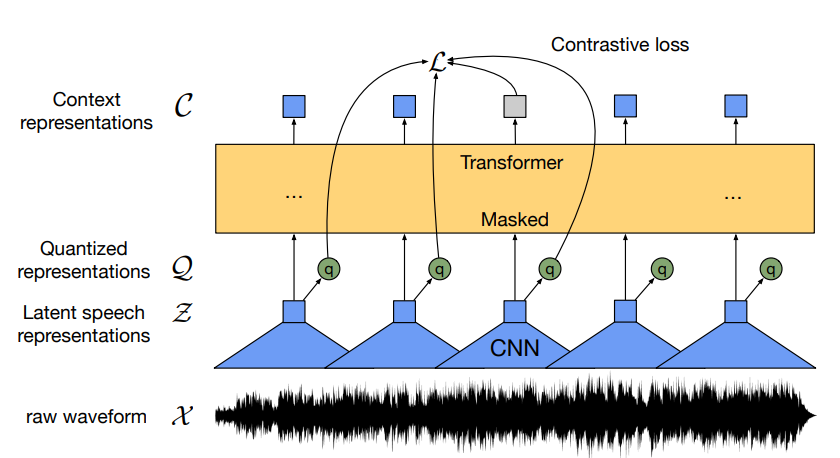
\includegraphics[width=0.7\textwidth]{figures/speech_representation_wav2vec2.PNG}
    \caption{\center{Illustration of wav2vec 2.0 framework which jointly learns contextualized speech representations
    \\and an inventory of discretized speech units.}}
    \label{speech_representation_wav2vec2}
    \end{figure}
    
\end{frame}


\begin{frame}{wav2vec 2.0 \cite{facebookwav2vec2}}

\begin{itemize}
    \item \textbf{Feature encoder}: Blocks of temporal convolution, layer normalization \cite{layer_normalization}, and the GELU activation function \cite{gelu}. 

    \item \textbf{Contextualized representations with Transformers}: A context network that uses the Transformer architecture \cite{Transformer}. 
    
    \item \textbf{Contrastive learning}: Get a context representation $c_t$ for a masked latent representation $z_t$ in order to guess the proper quantized representation $q_t$ among alternative quantized representations.

    \begin{figure}[hbtp]
    \centering
    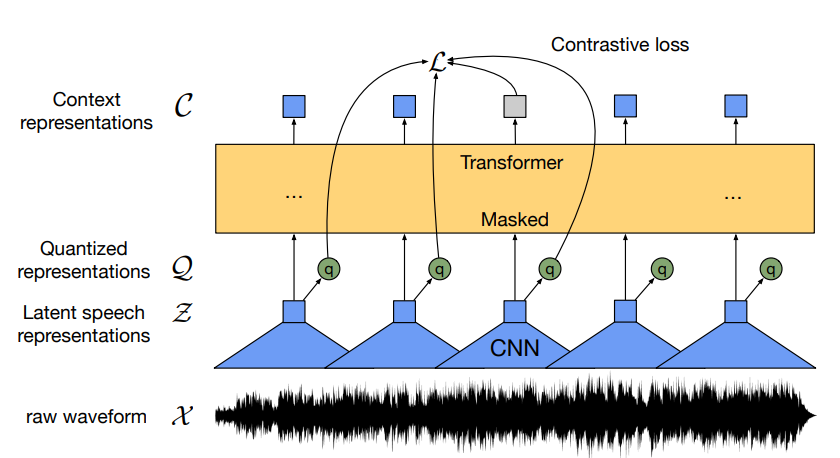
\includegraphics[width=0.5\textwidth]{figures/speech_representation_wav2vec2.PNG}
    \end{figure}
    
\end{itemize}

\end{frame}

% XLSR
\begin{frame}{Unsupervised cross-lingual representation learning (XLSR) \cite{XLSR}}

\begin{itemize}
    \item \textbf{XLSR}: By extending wav2vec 2.0 to the multilingual setting, cross-lingual learning seeks to create models that use data from other languages to improve performance. 
    
    \item \textbf{In-domain Match Level}:
     Determined by the similarity between recording conditions, naturalness and conversational topics.
    
    \item \textbf{Diversity Level}: of the multilingual dataset is higher than the monolingual one because the first represents more learnable phonemes helpful to target language.
\end{itemize}

\begin{figure}
    \centering
    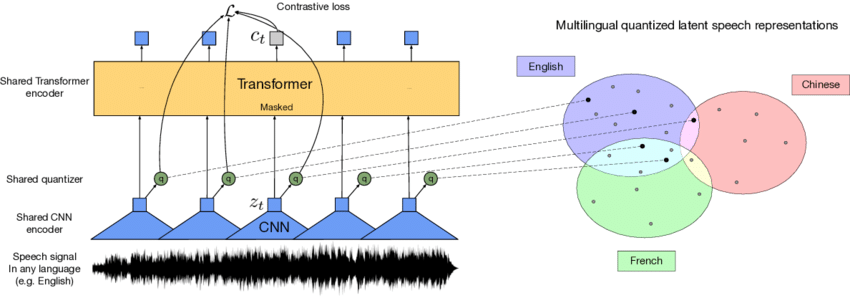
\includegraphics[width=0.8\textwidth]{xlsr_speech_representations.png}
\end{figure}
        
\end{frame}

\section{Experiments}

\begin{frame}{Training data}
\begin{itemize}
    \item Acoustic training data: %\TODO{Acoustic training data:}
\end{itemize}
\begin{table}[!h]
\captionsetup{font=Large}
\centering
\begin{adjustbox}{width=0.9\columnwidth,center}
\begin{tabular}{|l|c|c|c|c|c|c|c|} 
\hline
Language                    & Dataset                 & Usage                                                     & \# Spks & Hours  & Domain                                                                       & \begin{tabular}[c]{@{}c@{}}In-domain \\match\end{tabular} & \begin{tabular}[c]{@{}c@{}}Diversity \\level\end{tabular}  \\ 
\hline
Arabic                      & In-house                & pretr.                                                    & 3379    & 786    & Tel., Conv.                                                                  & Medium                                                    & Medium                                                     \\ 
\hline
German                      & In-house                & pretr.                                                    & 1723    & 177    & Tel., Conv.                                                                  & Medium                                                    & Medium                                                     \\ 
\hline
\multirow{5}{*}{Vietnamese} & In-house                & \begin{tabular}[c]{@{}c@{}}pretr., \\finetu.\end{tabular} & 2240    & 219    & Tel., Conv.                                                                  & Medium                                                    & Medium                                                     \\ 
\cline{2-8}
                            & \multirow{3}{*}{HYKIST} & adapt                                                     & 1       & 1      & \multirow{3}{*}{\begin{tabular}[c]{@{}c@{}}Tel., Conv.,\\Med.~\end{tabular}} & \multirow{3}{*}{High}                                     & \multirow{4}{*}{Low}                                       \\ 
\cline{3-5}
                            &                         & dev                                                       & 3       & 3      &                                                                              &                                                           &                                                            \\ 
\cline{3-5}
                            &                         & test                                                      & 2       & 2      &                                                                              &                                                           &                                                            \\ 
\cline{2-7}
                            & YouTube                 & pretr.                                                    & -       & 1.204  & Read books                                                                   & Low                                                       &                                                            \\ 
\hline
\multirow{2}{*}{Multi}      & In-house*               & pretr.                                                    & 7342    & 1.182  & Tel., Conv.                                                                  & Medium                                                    & \multirow{2}{*}{High}                                      \\ 
\cline{2-7}
                            & XLSR-53                 & pretr.                                                    & -       & 56.000 & Various                                                                      & Low                                                       &                                                            \\
\hline
\end{tabular}
\end{adjustbox}
\caption{\center{*The multilingual in-house training dataset is the combination of the Arabic, German and Vietnamese ones listed above. Domain: Telephone (Tel.), Conversational (Conv.), Medical (Med.). Sampling rate: 8kHz}}
\label{table:data_stats}
\end{table}

\end{frame}

\begin{frame}{Training data}
\begin{itemize}
    \item Data for the large out-of-domain recognition: Read speech datasets resampled from 16kHz to 8kHz: 
    \begin{itemize}
        \item CommonVoice Vietnamese (17h of noisy recordings) \cite{ardila2020commonvoice}
        \item VIVOS (15h of clean recordings) \cite{vivos_dataset}
    \end{itemize}
    \item Lexicon and language model:
\end{itemize}
% Please add the following required packages to your document preamble:
% \usepackage{multirow}
\begin{table}[!ht]
\setlength{\tabcolsep}{0.9em}
\centering
\begin{tabular}{|c|c|c|c|c|c|} 
\hline
\# words & vocab & \multicolumn{2}{c|}{dev} & \multicolumn{2}{c|}{test}  \\ 
\hline
in train & size  & OOV   & PPL              & OOV   & PPL                \\ 
\hline
500M     & 11k   & 0.1\% & 67               & 0.2\% & 69                 \\
\hline
\end{tabular}
\caption{ 4-gram LM for Vietnamese.}
\label{table:LM_stats}
\end{table}
 
\end{frame}

\begin{frame}{Acoustic model}
\begin{itemize}
    \item Supervised-only models: GMM, BLSTM (25M parameters), Transformer (90M)
    
    \item Models using unsupervised pretraining (317M by full architecture \textit{Large}, 115M parameters by cut-off \textit{Large}\textsubscript{1-8}\xspace \, and 95M by \textit{Base} architecture): 
    \begin{itemize}
        \item XLSR-53
        \item Models pretrained from scratch with custom data
        \item Continued pretraining with XLSR-53 as initialization
    \end{itemize}
    
    \item Regularization: 
    \begin{itemize}
        \item Unsupervised pretraining: 
        speed perturbation \cite{speed_perturbation}, random pitch perturbation \cite{pitch_perturbation}, reverberation perturbation \cite{reverb_perturbation}
        \item Finetuning: SpecAugment \cite{park2019specaugment}, Intermediate Cross-entropy Loss (ICE Loss), Intermediate Focal Loss (IF Loss), L2 Regularization \cite{L2_regularization}, On-off Regularization
    \end{itemize}
\end{itemize}
\end{frame}

\section{Experimental results}

% Supervised baselines and Monolingual pretraining

\begin{frame}{Supervised baselines}
    % Please add the following required packages to your document preamble:
% \usepackage{multirow}
\begin{table}[!ht]
\captionsetup{font=Large}
\centering
\begin{adjustbox}{width=0.5\columnwidth,center}
\begin{tabular}{|l|c|c|} 
\hline
\multicolumn{1}{|c|}{\multirow{2}{*}{AM}} & \multicolumn{2}{c|}{WER [\%]}  \\ 
\cline{2-3}
\multicolumn{1}{|c|}{}                    & Hykist dev & Hykist test       \\ 
\hline
GMM                                       & 62.2       & 59.7              \\ 
\hline
BLSTM                                     & 32.9       & 38.4              \\ 
\hline
Transformer                               & 31.0       & 35.1              \\
\hline
\end{tabular}
\end{adjustbox}
\caption{\center{\Glspl{WER} [\%] for supervised-only baselines on Vietnamese HYKIST data \cite{luescher2022:hykist}. 
\\ Models are trained on the monolingual in-house data.}}
\label{table:supervised_baselines}
%\TODO{the caption is very small}
\end{table}




\end{frame}

\begin{frame}{Monolingual pretraining}
% \usepackage{multirow}

\begin{table}[!ht]
\captionsetup{font=Large}
\centering
\begin{tabular}{|c|c|c|c|c|c|} 
\hline
\multicolumn{3}{|c|}{Pre-training}                                           & Fine-tuning         & \multicolumn{2}{c|}{WER [\%]}  \\ 
\hline
Data                          & ~Hours                & Epochs               & Epochs              & Hykist dev & Hykist test       \\ 
\hline
None                          & -                     & None                 & \multirow{2}{*}{33} & 32.1       & 36.6              \\ 
\cline{1-3}\cline{5-6}
Viet. in-house (sup. pret.)   & \multirow{2}{*}{219}  & 33                   &                     & 31.9       & 36.9              \\ 
\cline{1-1}\cline{3-6}
Viet. in-house (unsup. pret.) &                       & 100                  & \multirow{4}{*}{26} & 31.4       & 33.4              \\ 
\cline{1-3}\cline{5-6}
Aug. Viet. in-house           & \multirow{3}{*}{1168} & \multirow{3}{*}{300} &                     & 31.0       & 32.3              \\ 
\cline{1-1}\cline{5-6}
Viet. YT                      &                       &                      &                     & 29.8       & 35.2              \\ 
\cline{1-1}\cline{5-6}
Viet. in-house + YT           &                       &                      &                     & 25.3       & 27.2              \\
\hline
\end{tabular}
\caption{\center{All fine-tunings use the \textit{Large}\textsubscript{1-8} architecture and are trained until full convergence on Vietnamese in-house data and the recognition is done on HYKIST. All pre-trainings have been done with \textbf{random initialization}. Pre-training data "None" in the 3rd row means fine-tuning from scratch with wav2vec 2.0 \textit{Large}\textsubscript{1-8} architecture. 
In the experiment "supervised pretraining" in 4th row, we mimic the learning rate curve of the experiment "unsupervised pretraining" in 5th row.
The rest pretraining schedules are unsupervised.
The chosen number of pretraining epochs is the best checkpoint.}}
\label{table:monoling_pretraining}
%\TODO{add info: how much hours of data for fine tuning. in caption should suffice}
%\TODO{split | Data (hours) | $/rightarrow$ | Data | Hours |. I think that would make the table better readable}
%\TODO{move HYKIST label to WER or into a separate row??? might save a bit space in the width?}
\end{table}
\end{frame}    

\begin{frame}{Monolingual pretraining}
\begin{itemize}
    \item WERs of from scratch (32.1\% and 36.6\%) and in-house supervised pretraining (31.9\% and 36.9\%) reduce to (31.4\% and 33.4\%) of in-house pretraining 
    \\ \textrightarrow \, 
    On \textbf{wav2vec 2.0} architecture, the unsupervised pretraining helps 
    %\TODO{we don't have a control experiment where we trained longer thatn 33 epochs without pre-training, right?}
    
    \item WERs reduce from 31.4\% and 33.4\% to 31.0\% and 32.3\% 
    \\ \textrightarrow \,
    Data augmentation for pretraining is helpful
    
    \item WERs of Youtube data (29.8\% and 35.2\%) vs. in-house data (31.4\% and 33.4\%) 
    \\ \textrightarrow \,
    Having more data is not always helpful, if the domain mismatch is larger and the data has less speakers
    
    \item WERs by 25.3\% and 27.2\% when combining the in-house and YT data (the best result using solely monolingual data)
    \\ \textrightarrow \,
    Diversity of domains and speakers is necessary
\end{itemize}
%\TODO{these points need to be discussed with the table in view. so you need to say these things when you are showing the table, and then you can give a summary on the following slide}
\end{frame}

\begin{frame}{Multilingual pretraining}
    % \usepackage{multirow}

\begin{table}[!ht]
\centering
\begin{tabular}{|c|c|c|c|c|} 
\hline
\multicolumn{3}{|c|}{Pre-training}                                                                                       & \multicolumn{2}{c|}{WER [\%]}  \\ 
\hline
Init                    & Data (hours)                                                            & Epochs               & Hykist dev & Hykist test       \\ 
\hline
\multirow{2}{*}{random} & \begin{tabular}[c]{@{}c@{}}Viet. in-house + YT\\(1168h)\end{tabular}    & \multirow{2}{*}{300} & 25.3       & 27.2              \\ 
\cline{2-2}\cline{4-5}
                        & \begin{tabular}[c]{@{}c@{}}Multilingual in-house \\(1168h)\end{tabular} &                      & 26.8       & 28.7              \\ 
\hline
\textit{XLSR-53}\textsubscript{1-8}     & None                                                                    & None                 & 27.6       & 31.9              \\
\hline
\end{tabular}
\caption{\glspl{WER} {[}\%{]} for models using unsupervised pretraining on multilingual data compared to pretraining on monolingual data. All fine-tunings use the \textit{Large}\textsubscript{1-8} architecture and are trained until full convergence on Vietnamese in-house data and the recognition is done on HYKIST. The 2nd model is pretrained on our multilingual in-house dataset, and the 3rd uses \textit{XLSR-53}\textsubscript{1-8} to directly finetune on Vietnamese in-house data.}
\label{table:multiling_pretraining}
\end{table}
\end{frame}

\begin{frame}{Multilingual pretraining}
\begin{itemize}
    \item WERs of multilingual (26.8\% and 28.7\%) vs. monolingual combination (25.3\% and 27.2\%) 
    \\ \textrightarrow \, 
    Monolingual data with multiple domains outperforms multilingual data with high domain-match and speaker diversity.
    %We reject \cite{xlsr53}'s conclusion where multilingual pretraining is proved to outperform monolingual pretraining. \TODO{too strong! you don't have that many experiments. please talk to Julian to see what he has to say about this.}
        
    \item WERs by 27.6\% and 31.9\% when directly finetuning with \textit{XLSR-53} 
    \\ \textrightarrow \,
    May be due to the absence of 8kHz data in the pretraining of \textit{XLSR-53}
    %\TODO{why are you showing this experiment here? this is not clear to me. this is basically a supervised model or not?!}
\end{itemize}
\end{frame}
\section{Training time trade-offs in rapid development}

\begin{figure}[hbtp]
	\centering
	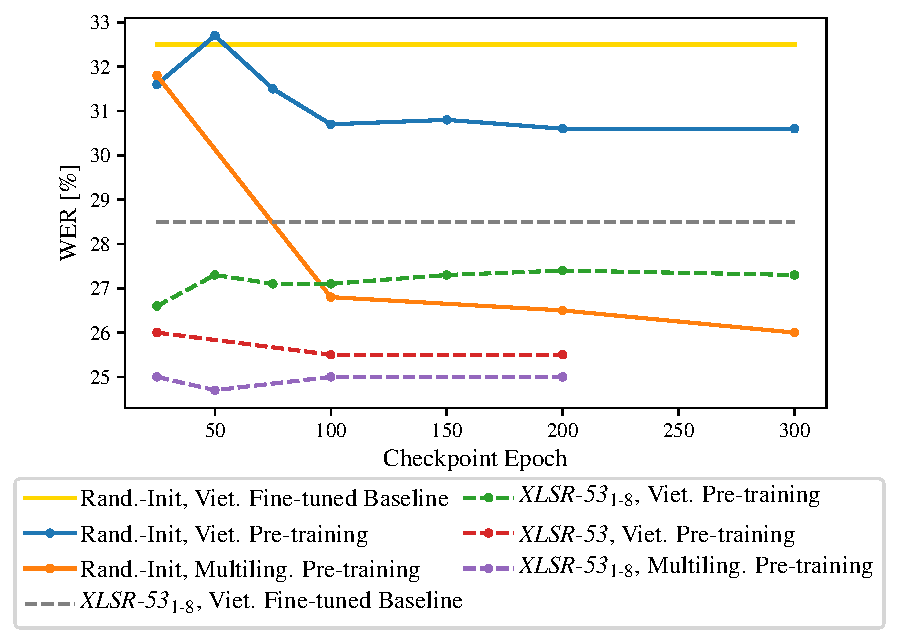
\includegraphics[width=1.0\textwidth]{figures/pretrain_comparison.pdf}
	\caption{
	    \glsxtrshort{WER} comparison using several pre-training checkpoints fine-tuned on the same schedule. 
	    The quantity of pre-training epochs is represented on the horizontal axis. 
	    The vertical axis displays the \glsxtrshort{WER} obtained after optimizing the Vietnamese in-house system on HYKIST dev data till convergence and evaluated on the initialization checkpoint that corresponds to it. 
	    All the pre-trainings in Vietnamese have been done using in-house data, not \glsxtrshort{YT} data. 
	    Keep in mind that if utilizing as an initialization, the training epochs for that model are not taken into consideration.
	    }
	\label{fig:fine_tune_comp_joint}
\end{figure}

It is vital to identify a trade-off between training time allowed and potential system performance while constructing \glsxtrshort{ASR} systems quickly. 
In this section, we examine the models that are most useful for this purpose. 
One epoch of pre-training on our internal Vietnamese data may be assumed to take around an hour on an NVIDIA 2080 GPU, but one epoch of fine-tuning can be estimated to take about three hours on the same setup. 
In our trials, the needed pre-training time scaled linearly with the amount of data.

Figure \ref{fig:fine_tune_comp_joint} compares various training methods using a hold-out dev dataset.
Yellow represents the baseline when fine-tuning from scratch.
Although pre-training using the in-house Vietnamese data (blue) results in a tiny improvement, it converges and stops improving after 100 iterations.
This is true even when the unsupervised loss is still improving.
Contrarily, the multilingual pre-training (orange) performs much better than the monolingual pre-training and enhances downstream \glsxtrshort{WER} even over prolonged training time.

Vietnamese \textit{XLSR-53}\textsubscript{1-8} (grey) fine-tuning is a very cost-effective training method that outperforms starting from scratch or pre-training on monolingual in-house data while utilizing only 26 training epochs in total.
Please take note that since the original \glsxtrshort{XLSR-53} model is available to the public, we do not count training epochs.
Although it requires more training time, using \glsxtrshort{XLSR-53} as an initialization for additional custom pre-training results in considerable \glsxtrshort{WERR} (green, red, purple).
It is evident from Figure \ref{fig:fine_tune_comp_joint} that even a brief pre-training with a few epochs produces significant benefits.
Consequently, this can be viewed as a quick and affordable solution to improve the performance of the model.
When employing data that is multilingual, the \glsxtrshort{WERR} is very potent.
Despite the fact that we have more data in this instance and a lengthier pre-training as a result, we only need to conduct this procedure once for all languages, making the situation essentially a zero-sum game.

In conclusion, it is clear that using the \glsxtrshort{XLSR-53} model to construct high-performing \glsxtrshort{ASR} models is very cost-effective. 
A quick multilingual pre-training that is helpful for downstream fine-tuning in all languages can further enhance performance.
\begin{frame}{Comparison to supervised baselines}
    % \usepackage{multirow}

\begin{table}[!ht]
\centering
\begin{tabular}{|c|c|c|c|c|} 
\hline
\multirow{2}{*}{AM}          & \multirow{2}{*}{Init}                & Pre-training                                                            & \multicolumn{2}{c|}{WER [\%]}  \\ 
\cline{3-5}
                             &                                      & Data (hours)                                                            & Hykist dev & Hykist test       \\ 
\hline
Transformer                  & \multirow{4}{*}{random}              & \multirow{2}{*}{None}                                                   & 31.0       & 35.1              \\ 
\cline{1-1}\cline{4-5}
\multirow{5}{*}{wav2vec 2.0} &                                      &                                                                         & 32.1       & 36.6              \\ 
\cline{3-5}
                             &                                      & \begin{tabular}[c]{@{}c@{}}Viet. in-house \\~(219h)\end{tabular}        & 31.4       & 33.4              \\ 
\cline{3-5}
                             &                                      & \begin{tabular}[c]{@{}c@{}}Viet. YT \\(1168h)\end{tabular}              & 29.8       & 35.2              \\ 
\cline{2-5}
                             & \multirow{2}{*}{\textit{XLSR-53}\textsubscript{1-8}} & \begin{tabular}[c]{@{}c@{}}Viet. in-house + YT \\(1168h)\end{tabular}   & 24.5       & 27.2              \\ 
\cline{3-5}
                             &                                      & \begin{tabular}[c]{@{}c@{}}Multilingual in-house~\\(1168h)\end{tabular} & 23.9       & 27.4              \\
\hline
\end{tabular}
\caption{\glspl{WER} {[}\%{]} for models using unsupervised pre-training and supervised-only training. All fine-tunings use the \textit{Large}\textsubscript{1-8} architecture and are trained until full convergence on Vietnamese in-house data and the recognition is done on HYKIST. The 1st model is the supervised-only training using Transformer. The 2nd and 3rd models are pretrained on specific data using random initializaton. The 4th and 5th models are continued pretraining methods (using \textit{XLSR-53}\textsubscript{1-8} as initialization).}
\label{table: supervised_unsupervised_compare}
\end{table}
\end{frame}

\begin{frame}{Comparison to supervised baselines}
\begin{itemize}
    \item WERs of in-house pretraining (31.4\% and 33.4\%) vs. YT data (29.8\% and 35.2\%) are higher than Transformer baseline (31.0\% and 35.1\%).
    \\ \textrightarrow \,
    wav2vec 2.0 unsupervised pretraining does not always outperform the Transformer supervised-only approach, especially when the pretrained data is not diverse enough.
    %\TODO{could it be that the amount of data is not enough for the model size? how big are Trafo and wav2vec2?}
    
    \item The best results are (24.5 \% and 27.2\%) on monolingual data and (23.9\% and 27.4\%) on multilingual data.
    \\ \textrightarrow \,
    Continued pretraining should be used regardless of sampling rate mismatch to gain the most benefits in terms of accuracy.
\end{itemize}
\end{frame}
\section{Effectiveness of intermediate loss}


\subsection{Effectiveness of Intermediate Cross-Entropy Loss}

%% \usepackage[normalem]{ulem}
% \usepackage{multirow}


\begin{table}[!ht]
\centering
\begin{adjustbox}{width=\columnwidth,center}
\begin{tabular}{|c|c|c|c|c|c|c|c|} 
\hline
Arch.                              & Init                              & Pre-training data                                                                    & Recog. & Baseline      & +ICE          & +IF           & +L2           \\ 
\hline
\multirow{8}{*}{\textit{Large}\textsubscript{1-8}} & \multirow{2}{*}{\textit{XLSR-53}}          & \multirow{2}{*}{None}                                                                & dev    & \textbf{27.9} & 28.4          & 28.0          & -             \\ 
\cline{4-8}
                                   &                                   &                                                                                      & test   & \textbf{32.3} & 33.3          & 32.8          & -             \\ 
\cline{2-8}
                                   & \multirow{4}{*}{None}             & \multirow{2}{*}{\begin{tabular}[c]{@{}c@{}}In-house data Viet.\\(219h)\end{tabular}} & dev    & 30.4          & 29.1          & \textbf{28.6} & 28.8          \\ 
\cline{4-8}
                                   &                                   &                                                                                      & test   & 33.4          & 33.7          & \textbf{33.0} & \uline{32.9}  \\ 
\cline{3-8}
                                   &                                   & \multirow{2}{*}{None}                                                                & dev    & 35.6          & 33.8          & \textbf{33.0} & \uline{31.4}  \\ 
\cline{4-8}
                                   &                                   &                                                                                      & test   & 40.7          & \textbf{38.1} & 38.8          & \uline{36.4}  \\ 
\cline{2-8}
                                   & \multirow{2}{*}{\textit{XLSR-53}} & \multirow{4}{*}{\begin{tabular}[c]{@{}c@{}}In-house data Viet.\\(219h)\end{tabular}} & dev    & 25.5          & 25.2          & \textbf{24.7} & \uline{24.3}  \\ 
\cline{4-8}
                                   &                                   &                                                                                      & test   & \textbf{29.1} & 29.2          & \textbf{29.1} & 29.3          \\ 
\cline{1-2}\cline{4-8}
\multirow{2}{*}{\textit{Base}}     & \multirow{4}{*}{None}             &                                                                                      & dev    & 30.2          & 29.7          & \textbf{29.0} & \uline{28.8}  \\ 
\cline{4-8}
                                   &                                   &                                                                                      & test   & 33.3          & 33.4          & \textbf{33.0} & \uline{32.3}  \\ 
\cline{1-1}\cline{3-8}
\multirow{2}{*}{\textit{Large}\textsubscript{1-8}} &                                   & \multirow{2}{*}{\begin{tabular}[c]{@{}c@{}}Viet. YT\\(1168h)\end{tabular}}           & dev    & 29.8          & 27.3          & \textbf{26.1} & -             \\ 
\cline{4-8}
                                   &                                   &                                                                                      & test   & 35.2          & 31.5          & \textbf{30.8} & -             \\
\hline
\end{tabular}
\end{adjustbox}
\caption{
    Comparison of \glspl{WER} between architecture sizes, pretrained datasets and pretrained models, all are finetuned on our in-house spontaneous telephone speech dataset and recognized at epoch 33 on dev and test telephone HYKIST data. 
    In this table, only 1 intermediate layer is applied in the middle \glsxtrshort{Transformer} block, e.g. position 4 for \textit{Large}\textsubscript{1-8} and 6 for \textit{Base} architecture. 
    \textbf{Bold} numbers are used to compare between the baseline and 2 types of intermediate loss, while \underline{underline} numbers denote extra improvement of L2 regularization compared to \glsxtrshort{IF Loss}}
\label{int_and_focal_WERs}
\end{table}
%\begin{table}[!ht]
\centering
\begin{adjustbox}{width=\columnwidth,center}
\begin{tabular}{|c|c|c|c|c|c|c|} 
\hline
Arch.                                                                      & Init                              & Pre-training data                                                                    & Recog. & Baseline      & +ICE           & +IF            \\ 
\hline
\multirow{12}{*}{\begin{tabular}[c]{@{}c@{}}\\\textit{Large}\textsubscript{1-8}\end{tabular}} & \multirow{3}{*}{\textit{XLSR-53}} & \multirow{3}{*}{None}                                                                & dev    & \textbf{14.8} & 15.8           & 15.4           \\ 
\cline{4-7}
                                                                           &                                   &                                                                                      & test   & \textbf{32.5} & 33.9           & 33.6           \\ 
\cline{4-7}
                                                                           &                                   &                                                                                      & vivos  & 30.3          & \textbf{30.0}  & \textbf{30.0}  \\ 
\cline{2-7}
                                                                           & \multirow{6}{*}{None}             & \multirow{3}{*}{In-house data Viet.(219h)}                                           & dev    & 16.4          & 16.1           & \textbf{15.8}  \\ 
\cline{4-7}
                                                                           &                                   &                                                                                      & test   & 35.6          & 34.8           & \textbf{34.5}  \\ 
\cline{4-7}
                                                                           &                                   &                                                                                      & vivos  & 31.3          & 30.4           & \textbf{29.6}  \\ 
\cline{3-7}
                                                                           &                                   & \multirow{3}{*}{None}                                                                & dev    & 20.8          & \textbf{18.6}  & 19.7           \\ 
\cline{4-7}
                                                                           &                                   &                                                                                      & test   & 44.7          & \textbf{42.1}  & 43.1           \\ 
\cline{4-7}
                                                                           &                                   &                                                                                      & vivos  & 34.9          & \textbf{33.1}  & 33.9           \\ 
\cline{2-7}
                                                                           & \multirow{3}{*}{\textit{XLSR-53}} & \multirow{6}{*}{\begin{tabular}[c]{@{}c@{}}In-house data Viet.\\(219h)\end{tabular}} & dev    & \textbf{11.5} & 12.3           & 13.0           \\ 
\cline{4-7}
                                                                           &                                   &                                                                                      & test   & \textbf{29.4} & 29.8           & 29.8           \\ 
\cline{4-7}
                                                                           &                                   &                                                                                      & vivos  & \textbf{27.2} & 27.7           & 27.6           \\ 
\cline{1-2}\cline{4-7}
\multirow{3}{*}{\textit{Base}}                                             & \multirow{6}{*}{None}             &                                                                                      & dev    & 16.6          & \textbf{15.4}~ & 15.9           \\ 
\cline{4-7}
                                                                           &                                   &                                                                                      & test   & 35.4          & \textbf{34.2}  & 34.4           \\ 
\cline{4-7}
                                                                           &                                   &                                                                                      & vivos  & 30.9          & 31.3           & \textbf{30.5}  \\ 
\cline{1-1}\cline{3-7}
\multirow{3}{*}{\begin{tabular}[c]{@{}c@{}}\\\textit{Large}\textsubscript{1-8}\end{tabular}}  &                                   & \multirow{3}{*}{Viet. YT(1168h)}                                                     & dev    & 16.4          & 15.6           & \textbf{14.5}  \\ 
\cline{4-7}
                                                                           &                                   &                                                                                      & test   & 34.4          & 32.2           & \textbf{30.9}  \\ 
\cline{4-7}
                                                                           &                                   &                                                                                      & vivos  & 28.7          & 27.6           & \textbf{26.9}  \\
\hline
\end{tabular}
\end{adjustbox}
\caption{
    Recognition \glspl{WER} at epoch 33 on read speech datasets. 
    Experiment setups are the same to Table \ref{int_and_focal_WERs}. 
    The recognition is done on CommonVoice dev/test sets and VIVOS test set.}
\label{int_and_focal_WERs_CV_Vivos}
\end{table}

\textbf{Improvement on HYKIST data}: In Table \ref{table:int_loss_hykist_pos}, when using in-house telephone dataset to train and transcribe the HYKIST dataset with the help of \glsxtrshort{ICE Loss}, we report the total improvement in performance for from scratch experiment where the \Glspl{WER} decrease from 35.6\% and 40.7\% to 33.8\% and 38.1\% on dev and test set respectively.
For \glsxtrshort{YT} experiment, the \Glspl{WER} decrease from 29.8\% and 35.2\% to 27.3\% and 31.5\%.
We also report a small improvement for the combination of Vietnamese in-house data and \glsxtrshort{YT} data, from 25.3\% and 27.2\% to 25.1\% and 27.1\%.

% \usepackage[normalem]{ulem}
% \usepackage{multirow}


\begin{table}[!ht]
\captionsetup{font=Large}
\centering
\begin{adjustbox}{width=0.8\columnwidth,center}
\begin{tabular}{|c|c|c|c|c|} 
\hline
\multicolumn{2}{|c|}{Pre-training}                           & \multirow{2}{*}{With ICE} & \multicolumn{2}{c|}{WER [\%]}  \\ 
\cline{1-2}\cline{4-5}
Data                                 & Hours                 &                           & Hykist dev & Hykist test       \\ 
\hline
\multirow{2}{*}{None}                & \multirow{2}{*}{-}    & No                        & 35.6       & 40.7              \\ 
\cline{3-5}
                                     &                       & Yes                       & 33.8       & 38.1              \\ 
\hline
\multirow{2}{*}{Viet. YT}            & \multirow{4}{*}{1168} & No                        & 29.8       & 35.2              \\ 
\cline{3-5}
                                     &                       & Yes                       & 27.3       & 31.5              \\ 
\cline{1-1}\cline{3-5}
\multirow{2}{*}{Viet. in-house + YT} &                       & No                        & 25.3       & 27.2              \\ 
\cline{3-5}
                                     &                       & Yes                       & 25.1       & 27.1              \\
\hline
\end{tabular}
\end{adjustbox}
\caption{
    \center{Improvements of WERs on HYKIST data between pretraining schedules when applying ICE Loss. 
    All pretrainings use the \textit{Large}\textsubscript{1-8} architecture with random initialization and are finetuned until full convergence on Vietnamese in-house data. 
    Only 1 intermediate layer is applied in the middle Transformer block, e.g. position 4 for \textit{Large}\textsubscript{1-8} and 6 for \textit{Base} architecture.}}
\label{table:int_loss_hykist_pos}
\end{table}

\textbf{Degradation on HYKIST data}: As shown in Table \ref{table:int_loss_hykist_neg}, for the directly finetuning experiment with \glsxtrshort{XLSR-53} preloaded, the performance is hurt totally (both \Glspl{WER} on dev and test sets increase).
Besides, both continued pretrainings on Vietnamese in-house and on \glsxtrshort{YT} data experience the partial improvements (only \Glspl{WER} on test sets are slightly increased but \Glspl{WER} on dev sets decrease).
The rest pretraining schedules in Table \ref{table:int_loss_hykist_neg} also experience partial improvements.

% \usepackage[normalem]{ulem}
% \usepackage{multirow}


\begin{table}[!ht]
\centering
\begin{adjustbox}{width=\columnwidth,center}
\begin{tabular}{|c|c|c|c|c|c|} 
\hline
\multirow{2}{*}{Arch.}         & \multirow{2}{*}{Init.}             & \multirow{2}{*}{Pre-training data}                                                    & \multirow{2}{*}{With ICE} & \multicolumn{2}{c|}{WER [\%]}  \\ 
\cline{5-6}
                               &                                    &                                                                                       &                           & Hykist dev & Hykist test       \\ 
\hline
\multirow{6}{*}{\textit{Large}\textsubscript{1-8}}      & \multirow{2}{*}{\textit{XLSR-53}}  & \multirow{2}{*}{None}                                                                 & No                        & 27.9       & 32.3              \\ 
\cline{4-6}
                               &                                    &                                                                                       & Yes                       & 28.4       & 33.3              \\ 
\cline{2-6}
                               & \multirow{2}{*}{None}              & \multirow{6}{*}{\begin{tabular}[c]{@{}c@{}}Viet. in-house\\(219h)\end{tabular}}       & No                        & 30.4       & 33.4              \\ 
\cline{4-6}
                               &                                    &                                                                                       & Yes                       & 29.1       & 33.7              \\ 
\cline{2-2}\cline{4-6}
                               & \multirow{2}{*}{\textit{XLSR-53 }} &                                                                                       & No                        & 25.5       & 29.1              \\ 
\cline{4-6}
                               &                                    &                                                                                       & Yes                       & 25.2       & 29.2              \\ 
\cline{1-2}\cline{4-6}
\multirow{2}{*}{\textit{Base}} & \multirow{4}{*}{None}              &                                                                                       & No                        & 30.2       & 33.3              \\ 
\cline{4-6}
                               &                                    &                                                                                       & Yes                       & 29.7       & 33.4              \\ 
\cline{1-1}\cline{3-6}
\multirow{4}{*}{\textit{Large}\textsubscript{1-8}}      &                                    & \multirow{2}{*}{\begin{tabular}[c]{@{}c@{}}Multiling. in-house\\(1168h)\end{tabular}} & No                        & 26.8       & 28.7              \\ 
\cline{4-6}
                               &                                    &                                                                                       & Yes                       & 25.5       & 29.4              \\ 
\cline{2-6}
                               & \multirow{2}{*}{\textit{XLSR-53}}  & \multirow{2}{*}{\begin{tabular}[c]{@{}c@{}}Viet. YT\\(1168h)\end{tabular}}            & No                        & 24.3       & 28.1              \\ 
\cline{4-6}
                               &                                    &                                                                                       & Yes                       & 23.7       & 28.2              \\
\hline
\end{tabular}
\end{adjustbox}
\caption{
    Degradations of \glspl{WER} {[}\%{]} on HYKIST data between pretraining schedules when applying \glsxtrshort{ICE Loss}. All models are finetuned until full convergence on Vietnamese in-house data. 
    Only 1 intermediate layer is applied in the middle \glsxtrshort{Transformer} block, e.g. position 4 for \textit{Large}\textsubscript{1-8} and 6 for \textit{Base} architecture.
    }
\label{table:int_loss_hykist_neg}
\end{table}

\textbf{Improvement on CommonVoice and VIVOS data}: In the situation of more out-of-domain recognition shown in Table \ref{int_loss_cvvivos_pos}, which means using the model finetuned on our in-house spontaneous telephone speech dataset to do the recognition on read speech datasets like CommonVoice and VIVOS, we report the total improvements in performance for \textit{Large}\textsubscript{1-8} in-house pretraining, from scratch and \glsxtrshort{YT} experiments. 
Notable is from scratch training where \glsxtrshort{WER}s reduce from 20.8\%, 44.7\%, 34.9\% to 18.6\%, 42.1\%, 33.1\%; and \glsxtrshort{YT} pretraining where \glsxtrshort{WER}s reduce from 16.4\%, 34.4\%, 28.7\% to 15.6\%, 32.2\%, 27.6\% on CommonVoice dev/test and VIVOS test set respectively.
Together with the improvements on HYKIST reported in Table \ref{table:int_loss_hykist_pos}, we conclude that using \glsxtrshort{ICE Loss} for from scratch training and for pretraining on \glsxtrshort{YT} data improves the recognitions on both telephone and read speech domain.

\begin{table}[!ht]
\captionsetup{font=Large}
\centering
\begin{adjustbox}{width=0.7\columnwidth,center}
\begin{tabular}{|c|c|c|c|c|c|} 
\hline
\multicolumn{2}{|c|}{Pre-training}                      & \multirow{2}{*}{With ICE} & \multicolumn{3}{c|}{WER [\%]}  \\ 
\cline{1-2}\cline{4-6}
Data                            & Hours                 &                           & CV dev & CV test & Vivos       \\ 
\hline
\multirow{2}{*}{None}           & \multirow{2}{*}{-}    & No                        & 20.8   & 44.7    & 34.9        \\ 
\cline{3-6}
                                &                       & Yes                       & 18.6   & 42.1    & 33.1        \\ 
\hline
\multirow{2}{*}{Viet. YT}       & \multirow{2}{*}{1168} & No                        & 16.4   & 34.4    & 28.7        \\ 
\cline{3-6}
                                &                       & Yes                       & 15.6   & 32.2    & 27.6        \\ 
\hline
\multirow{2}{*}{Viet. in-house} & \multirow{2}{*}{219}  & No                        & 16.4   & 35.6    & 31.3        \\ 
\cline{3-6}
                                &                       & Yes                       & 16.1   & 34.8    & 30.4        \\
\hline
\end{tabular}
\end{adjustbox}
\caption{
    \center{Improvements of WERs on CommonVoice and VIVOS between pretraining schedules when applying ICE Loss.
    All pretrainings use the \textit{Large}\textsubscript{1-8} architecture with random initialization and are finetuned until full convergence on Vietnamese in-house data.}}
\label{int_loss_cvvivos_pos}
\end{table}

\textbf{Degradation on CommonVoice and VIVOS data}: As shown in the Table \ref{int_loss_cvvivos_neg}, we experience the total degradations for 2 cases: continued pretraining on Vietnamese in-house data and pretraining on the combination of in-house and \glsxtrshort{YT} data; where \glsxtrshort{WER}s for all read speech test sets increase.
The rest cases experience partial degradations.

\begin{table}[!ht]
\captionsetup{font=Large}
\centering
\begin{adjustbox}{width=0.8\columnwidth,center}
\begin{tabular}{|c|c|c|c|c|c|c|c|} 
\hline
\multirow{2}{*}{Arch.}             & \multirow{2}{*}{Init.}            & \multicolumn{2}{c|}{Pre-training}                            & \multirow{2}{*}{With ICE} & \multicolumn{3}{c|}{WER [\%]}  \\ 
\cline{3-4}\cline{6-8}
                                   &                                   & Data                                 & Hours                 &                           & CV dev & CV test & Vivos       \\ 
\hline
\multirow{4}{*}{\textit{Large}\textsubscript{1-8}} & \multirow{4}{*}{\textit{XLSR-53}} & \multirow{2}{*}{None}                & \multirow{2}{*}{-}    & No                        & 14.8   & 32.5    & 30.3        \\ 
\cline{5-8}
                                   &                                   &                                      &                       & Yes                       & 15.8   & 33.9    & 30.0        \\ 
\cline{3-8}
                                   &                                   & \multirow{4}{*}{Viet. in-house}      & \multirow{4}{*}{219}  & No                        & 11.5   & 29.4    & 27.2        \\ 
\cline{5-8}
                                   &                                   &                                      &                       & Yes                       & 12.3   & 29.8    & 27.7        \\ 
\cline{1-2}\cline{5-8}
\multirow{2}{*}{\textit{Base}}     & \multirow{6}{*}{None}             &                                      &                       & No                        & 16.6   & 35.4    & 30.9        \\ 
\cline{5-8}
                                   &                                   &                                      &                       & Yes                       & 15.4   & 34.2    & 31.3        \\ 
\cline{1-1}\cline{3-8}
\multirow{6}{*}{\textit{Large}\textsubscript{1-8}} &                                   & \multirow{2}{*}{Multiling. in-house} & \multirow{6}{*}{1168} & No                        & 15.2   & 29.7    & 29.5        \\ 
\cline{5-8}
                                   &                                   &                                      &                       & Yes                       & 14.8   & 30.5    & 28.8        \\ 
\cline{3-3}\cline{5-8}
                                   &                                   & \multirow{2}{*}{Viet. in-house + YT} &                       & No                        & 12.9   & 26.5    & 21.0        \\ 
\cline{5-8}
                                   &                                   &                                      &                       & Yes                       & 13.6   & 28.2    & 21.9        \\ 
\cline{2-3}\cline{5-8}
                                   & \multirow{2}{*}{\textit{XLSR-53}} & \multirow{2}{*}{Viet. YT}            &                       & No                        & 11.8   & 28.4    & 25.6        \\ 
\cline{5-8}
                                   &                                   &                                      &                       & Yes                       & 12.3   & 28.3    & 25.0        \\
\hline
\end{tabular}
\end{adjustbox}
\caption{
    \center{Degradations of WERs on CommonVoice and VIVOS between pretraining schedules when applying ICE Loss.}}
\label{int_loss_cvvivos_neg}
\end{table}

\bigskip

\subsection{Effectiveness of Intermediate Focal Loss}

\textbf{Effectiveness on HYKIST data}: 

As shown in Table \ref{table:if_loss_hykist_pos} and Table \ref{table:if_loss_hykist_neg} below, when using \glsxtrshort{IF Loss}, we see the \Glspl{WER} on HYKIST improved compared to the baselines for various pretraining schedules (7/9 experiments experience total improvements), compared to only 3/9 experiments experiencing total improvements using \glsxtrshort{ICE Loss} (\glsxtrshort{ICE Loss} results are shown in Table \ref{table:int_loss_hykist_pos} and Table \ref{table:int_loss_hykist_neg} above).
In addition, we report all \Glspl{WER} of \glsxtrshort{IF Loss} experiments to be lower than those of \glsxtrshort{ICE Loss} experiments, except the one on HYKIST test set of from scratch training. 
We therefore conclude that, when finetuning and recognizing on the same telephone domain, \glsxtrshort{IF Loss} works better than \glsxtrshort{ICE Loss}. 

Compared to our strongest continued pretraining baseline, the application of \glsxtrshort{IF Loss} on the combination of Vietnamese in-house and \glsxtrshort{YT} data (24.5\% and 27.1\%) outperforms the results of continued pretraining on the combination of Vietnamese in-house and \glsxtrshort{YT} data (24.5\% and 27.2\% on dev and test set respectively as shown in Table \ref{table: xlsr53_init_pretrain}).
However, we believe that the \glsxtrshort{IF Loss} can further reduce \glsxtrshort{WER}s for this continued pretraining schedule, as it does with continued pretraining on \glsxtrshort{YT} data. 

Among all total improvements reported in Table \ref{table:if_loss_hykist_pos}, notable is the \Glspl{WER} reduction of \glsxtrshort{YT} experiment from 29.8\% and 35.2\% to 26.1\% and 30.8\% on dev and test set respectively, whose relative \glsxtrshort{WERR} is around 12.5\% in average.
For a more diverse pretrained data (Vietnamese in-house data), we report the \glsxtrshort{WER}s reduction from 30.4\% and 33.4\% to 28.6\% and 33.0\%, whose relative \glsxtrshort{WERR} is around 3.6\% in average.
For even more diverse pretrained data (Vietnamese in-house  + \glsxtrshort{YT} data), we report the \glsxtrshort{WER}s reduction from 25.3\% and 27.2\% to 24.5\% and 27.1\%, whose relative \glsxtrshort{WERR} is around 1.8\% in average.
We therefore conclude that the effectiveness of \glsxtrshort{IF Loss} decreases when the pretrained data becomes more diverse.


% \usepackage[normalem]{ulem}
% \usepackage{multirow}


\begin{table}[!ht]
\centering
\begin{adjustbox}{width=\columnwidth,center}
\begin{tabular}{|c|c|c|c|c|c|} 
\hline
\multirow{2}{*}{Arch.}             & \multirow{2}{*}{Init.}             & \multirow{2}{*}{Pre-training data}                                                    & \multirow{2}{*}{With IF} & \multicolumn{2}{c|}{WER [\%]}  \\ 
\cline{5-6}
                                   &                                    &                                                                                       &                          & Hykist dev & Hykist test       \\ 
\hline
\multirow{6}{*}{\textit{Large}\textsubscript{1-8}} & \multirow{4}{*}{None}              & \multirow{2}{*}{None}                                                                 & No                       & 35.6       & 40.7              \\ 
\cline{4-6}
                                   &                                    &                                                                                       & Yes                      & 33.0       & 38.8              \\ 
\cline{3-6}
                                   &                                    & \multirow{6}{*}{\begin{tabular}[c]{@{}c@{}}Viet. in-house\\(219h)\end{tabular}}       & No                       & 30.4       & 33.4              \\ 
\cline{4-6}
                                   &                                    &                                                                                       & Yes                      & 28.6       & 33.0              \\ 
\cline{2-2}\cline{4-6}
                                   & \multirow{2}{*}{\textit{XLSR-53 }} &                                                                                       & No                       & 25.5       & 29.1              \\ 
\cline{4-6}
                                   &                                    &                                                                                       & Yes                      & 24.7       & 29.1              \\ 
\cline{1-2}\cline{4-6}
\multirow{2}{*}{\textit{Base}}     & \multirow{6}{*}{None}              &                                                                                       & No                       & 30.2       & 33.3              \\ 
\cline{4-6}
                                   &                                    &                                                                                       & Yes                      & 29.0       & 33.0              \\ 
\cline{1-1}\cline{3-6}
\multirow{6}{*}{\textit{Large}\textsubscript{1-8}} &                                    & \multirow{2}{*}{\begin{tabular}[c]{@{}c@{}}Viet. YT\\(1168h)\end{tabular}}            & No                       & 29.8       & 35.2              \\ 
\cline{4-6}
                                   &                                    &                                                                                       & Yes                      & 26.1       & 30.8              \\ 
\cline{3-6}
                                   &                                    & \multirow{2}{*}{\begin{tabular}[c]{@{}c@{}}Viet. in-house + YT\\(1168h)\end{tabular}} & No                       & 25.3       & 27.2              \\ 
\cline{4-6}
                                   &                                    &                                                                                       & Yes                      & 24.5       & 27.1              \\ 
\cline{2-6}
                                   & \multirow{2}{*}{\textit{XLSR-53}}  & \multirow{2}{*}{\begin{tabular}[c]{@{}c@{}}Viet. YT\\(1168h)\end{tabular}}            & No                       & 24.3       & 28.1              \\ 
\cline{4-6}
                                   &                                    &                                                                                       & Yes                      & 23.4       & 28.1              \\
\hline
\end{tabular}
\end{adjustbox}
\caption{
    Improvements of \glspl{WER} {[}\%{]} on HYKIST data between pretraining schedules when applying \glsxtrshort{IF Loss}. All models are finetuned until full convergence on Vietnamese in-house data. 
    Only 1 intermediate layer is applied in the middle \glsxtrshort{Transformer} block, e.g. position 4 for \textit{Large}\textsubscript{1-8} and 6 for \textit{Base} architecture.}
\label{table:if_loss_hykist_pos}
\end{table}

As shown in Table \ref{table:if_loss_hykist_neg}, only for the case of directly finetuning with \glsxtrshort{XLSR-53}, using \glsxtrshort{IF Loss} makes the \Glspl{WER} on HYKIST increased compared to the baselines. 
However, the degradation is rather small, from 27.9\% and 32.3\% to 28.0\% and 32.8\% on dev and test set respectively.
Besides, a partial degradation of performance is reported in the multilingual in-house data experiment, where the  average \glsxtrshort{WER} of dev and test set (25.2\% and 29.3\%) is even lower than the baseline (26.8\% and 28.7\%).
Hence, in a rapid deployment of an \glsxtrshort{ASR} system, we recommend the direct use of \glsxtrshort{IF Loss} in training without the need of one more training as a baseline for performance comparison.

% \usepackage[normalem]{ulem}
% \usepackage{multirow}


\begin{table}[!ht]
\captionsetup{font=Large}
\centering
\begin{adjustbox}{width=0.7\columnwidth,center}
\begin{tabular}{|c|c|c|c|c|c|} 
\hline
\multirow{2}{*}{Init.}            & \multicolumn{2}{c|}{Pre-training}                            & \multirow{2}{*}{With IF} & \multicolumn{2}{c|}{WER [\%]}  \\ 
\cline{2-3}\cline{5-6}
                                  & Data                                 & Hours                 &                          & Hykist dev & Hykist test       \\ 
\hline
\multirow{2}{*}{\textit{XLSR-53}} & \multirow{2}{*}{None}                & \multirow{2}{*}{-}    & No                       & 27.9       & 32.3              \\ 
\cline{4-6}
                                  &                                      &                       & Yes                      & 28.0       & 32.8              \\ 
\hline
\multirow{2}{*}{None}             & \multirow{2}{*}{Multiling. in-house} & \multirow{2}{*}{1168} & No                       & 26.8       & 28.7              \\ 
\cline{4-6}
                                  &                                      &                       & Yes                      & 25.2       & 29.3              \\
\hline
\end{tabular}
\end{adjustbox}
\caption{
    \center{Degradations of WERs on HYKIST data between pretraining schedules when applying IF Loss.
    All pretrainings use the \textit{Large}\textsubscript{1-8} architecture and are finetuned until full convergence on Vietnamese in-house data.}}
\label{table:if_loss_hykist_neg}
\end{table}

\bigskip

\textbf{Effectiveness on CommonVoice and VIVOS data}: 

In the larger domain-shift recognition, we still receive the significant reduction of \Glspl{WER} in multiple experiments as shown in Table \ref{table:if_loss_cvvivos_pos}. 
The notable reduction of \Glspl{WER} compared to baselines is again on \glsxtrshort{YT} data, whose \Glspl{WER}s decrease from 16.4\%, 34.4\% and 28.7\% to 14.5\%, 30.9\% and 26.9\% respectively for 3 read speech sets, that makes \glsxtrshort{WERR} about 9.3\% in average.
The \glsxtrshort{ICE Loss} in Table \ref{int_loss_cvvivos_pos} makes 3 experiments totally improved, while the \glsxtrshort{IF Loss} makes 4. 
Furthermore, the \glsxtrshort{WER}s for \glsxtrshort{IF Loss} on 3 read speech datasets are as competitive as \glsxtrshort{ICE Loss}.
In addition, when finetuning and recognizing on the same telephone domain, \glsxtrshort{IF Loss} works better than \glsxtrshort{ICE Loss} as proved above.
We therefore conclude that \glsxtrshort{IF Loss} works better than \glsxtrshort{ICE Loss} in all domains.

\begin{table}[!ht]
\captionsetup{font=Large}
\centering
\begin{adjustbox}{width=0.8\columnwidth,center}
\begin{tabular}{|c|c|c|c|c|c|c|} 
\hline
\multirow{2}{*}{Arch.}             & \multicolumn{2}{c|}{Pre-training}                       & \multirow{2}{*}{With IF} & \multicolumn{3}{c|}{WER [\%]}  \\ 
\cline{2-3}\cline{5-7}
                                   & Data                            & Hours                 &                          & CV dev & CV test & Vivos       \\ 
\hline
\multirow{4}{*}{\textit{Large}\textsubscript{1-8}} & \multirow{2}{*}{Viet. in-house} & \multirow{2}{*}{219}  & No                       & 16.4   & 35.6    & 31.3        \\ 
\cline{4-7}
                                   &                                 &                       & Yes                      & 15.8   & 34.5    & 29.6        \\ 
\cline{2-7}
                                   & \multirow{2}{*}{None}           & \multirow{2}{*}{-}    & No                       & 20.8   & 44.7    & 34.9        \\ 
\cline{4-7}
                                   &                                 &                       & Yes                      & 19.7   & 43.1    & 33.9        \\ 
\hline
\multirow{2}{*}{\textit{Base}}     & \multirow{2}{*}{Viet. in-house} & \multirow{2}{*}{219}  & No                       & 16.6   & 35.4    & 30.9        \\ 
\cline{4-7}
                                   &                                 &                       & Yes                      & 15.9   & 34.4    & 30.5        \\ 
\hline
\multirow{2}{*}{\textit{Large}\textsubscript{1-8}} & \multirow{2}{*}{Viet. YT}       & \multirow{2}{*}{1168} & No                       & 16.4   & 34.4    & 28.7        \\ 
\cline{4-7}
                                   &                                 &                       & Yes                      & 14.5   & 30.9    & 26.9        \\
\hline
\end{tabular}
\end{adjustbox}
\caption{
    \center{Improvements of WERs on CommonVoice and VIVOS between pretraining schedules when applying IF Loss.
    All models are finetuned until full convergence on Vietnamese in-house data.}}
\label{table:if_loss_cvvivos_pos}
\end{table}

However, in the larger domain-shift recognition, we still meet degradations of performance in experiments pretrained on diverse data, as shown in Table \ref{table:if_loss_cvvivos_neg}.
We therefore recommend the use of \glsxtrshort{IF Loss} only for less diverse pretrained data if the domain of finetuning and recognition data are too different.

\begin{table}[!ht]
\centering
\begin{adjustbox}{width=0.9\columnwidth,center}
\begin{tabular}{|c|c|c|c|c|c|} 
\hline
\multirow{2}{*}{Init.}            & \multirow{2}{*}{Pre-training data}                                                    & \multirow{2}{*}{With IF} & \multicolumn{3}{c|}{WER [\%]}  \\ 
\cline{4-6}
                                  &                                                                                       &                          & CV dev & CV test & Vivos       \\ 
\hline
\multirow{4}{*}{\textit{XLSR-53}} & \multirow{2}{*}{None}                                                                 & No                       & 14.8   & 32.5    & 30.3        \\ 
\cline{3-6}
                                  &                                                                                       & Yes                      & 15.4   & 33.6    & 30.0        \\ 
\cline{2-6}
                                  & \multirow{2}{*}{\begin{tabular}[c]{@{}c@{}}Viet. in-house\\(219h)\end{tabular}}       & No                       & 11.5   & 29.4    & 27.2        \\ 
\cline{3-6}
                                  &                                                                                       & Yes                      & 13.0   & 29.8    & 27.6        \\ 
\hline
\multirow{4}{*}{None}             & \multirow{2}{*}{\begin{tabular}[c]{@{}c@{}}Multiling. in-house\\(1168h)\end{tabular}} & No                       & 15.2   & 29.7    & 29.5        \\ 
\cline{3-6}
                                  &                                                                                       & Yes                      & 14.5   & 30.6    & 28.1        \\ 
\cline{2-6}
                                  & \multirow{2}{*}{\begin{tabular}[c]{@{}c@{}}Viet. in-house + YT\\(1168h)\end{tabular}} & No                       & 12.9   & 26.5    & 21.0        \\ 
\cline{3-6}
                                  &                                                                                       & Yes                      & 12.7   & 28.6    & 22.1        \\ 
\hline
\multirow{2}{*}{\textit{XLSR-53}} & \multirow{2}{*}{\begin{tabular}[c]{@{}c@{}}Viet. YT\\(1168h)\end{tabular}}            & No                       & 11.8   & 28.4    & 25.6        \\ 
\cline{3-6}
                                  &                                                                                       & Yes                      & 13.2   & 29.1    & 24.5        \\
\hline
\end{tabular}
\end{adjustbox}
\caption{
    Degradations of \glspl{WER} {[}\%{]} on CommonVoice and VIVOS between pretraining schedules when applying \glsxtrshort{IF Loss}. All models are finetuned on Vietnamese in-house data. 
    Only 1 intermediate layer is applied in the middle \glsxtrshort{Transformer} block, e.g. position 4 for \textit{Large}\textsubscript{1-8} and 6 for \textit{Base} architecture.}
\label{table:if_loss_cvvivos_neg}
\end{table}

\begin{frame}{Effectiveness of Intermediate Cross-Entropy Loss}
\begin{itemize}
    \item Improvement on HYKIST data: Total improvements for 3/9 experiments of small out-of-domain recognition
\end{itemize}
% \usepackage[normalem]{ulem}
% \usepackage{multirow}


\begin{table}[!ht]
\captionsetup{font=Large}
\centering
\begin{adjustbox}{width=0.8\columnwidth,center}
\begin{tabular}{|c|c|c|c|c|} 
\hline
\multicolumn{2}{|c|}{Pre-training}                           & \multirow{2}{*}{With ICE} & \multicolumn{2}{c|}{WER [\%]}  \\ 
\cline{1-2}\cline{4-5}
Data                                 & Hours                 &                           & Hykist dev & Hykist test       \\ 
\hline
\multirow{2}{*}{None}                & \multirow{2}{*}{-}    & No                        & 35.6       & 40.7              \\ 
\cline{3-5}
                                     &                       & Yes                       & 33.8       & 38.1              \\ 
\hline
\multirow{2}{*}{Viet. YT}            & \multirow{4}{*}{1168} & No                        & 29.8       & 35.2              \\ 
\cline{3-5}
                                     &                       & Yes                       & 27.3       & 31.5              \\ 
\cline{1-1}\cline{3-5}
\multirow{2}{*}{Viet. in-house + YT} &                       & No                        & 25.3       & 27.2              \\ 
\cline{3-5}
                                     &                       & Yes                       & 25.1       & 27.1              \\
\hline
\end{tabular}
\end{adjustbox}
\caption{
    \center{Improvements of WERs on HYKIST data between pretraining schedules when applying ICE Loss. 
    All pretrainings use the \textit{Large}\textsubscript{1-8} architecture with random initialization and are finetuned until full convergence on Vietnamese in-house data. 
    Only 1 intermediate layer is applied in the middle Transformer block, e.g. position 4 for \textit{Large}\textsubscript{1-8} and 6 for \textit{Base} architecture.}}
\label{table:int_loss_hykist_pos}
\end{table}
%\TODO{why are you only showing the results where this works? you have to show all results! Otherwise you are handpicking results which means this is not conclusive at all.}
%\TODO{The tables for ICE and IF should look the same: slides 27, 28, 29, 31, 32}
%\TODO{what could be the reason for ICE helping in certain conditions?}
\end{frame}


\begin{frame}{Effectiveness of Intermediate Cross-Entropy Loss}
\begin{itemize}
    \item Degradation on HYKIST data: Total degradation for directly finetuning with \textit{XLSR-53}. The rest are partial degradations.
\end{itemize}
% \usepackage[normalem]{ulem}
% \usepackage{multirow}


\begin{table}[!ht]
\centering
\begin{adjustbox}{width=\columnwidth,center}
\begin{tabular}{|c|c|c|c|c|c|} 
\hline
\multirow{2}{*}{Arch.}         & \multirow{2}{*}{Init.}             & \multirow{2}{*}{Pre-training data}                                                    & \multirow{2}{*}{With ICE} & \multicolumn{2}{c|}{WER [\%]}  \\ 
\cline{5-6}
                               &                                    &                                                                                       &                           & Hykist dev & Hykist test       \\ 
\hline
\multirow{6}{*}{\textit{Large}\textsubscript{1-8}}      & \multirow{2}{*}{\textit{XLSR-53}}  & \multirow{2}{*}{None}                                                                 & No                        & 27.9       & 32.3              \\ 
\cline{4-6}
                               &                                    &                                                                                       & Yes                       & 28.4       & 33.3              \\ 
\cline{2-6}
                               & \multirow{2}{*}{None}              & \multirow{6}{*}{\begin{tabular}[c]{@{}c@{}}Viet. in-house\\(219h)\end{tabular}}       & No                        & 30.4       & 33.4              \\ 
\cline{4-6}
                               &                                    &                                                                                       & Yes                       & 29.1       & 33.7              \\ 
\cline{2-2}\cline{4-6}
                               & \multirow{2}{*}{\textit{XLSR-53 }} &                                                                                       & No                        & 25.5       & 29.1              \\ 
\cline{4-6}
                               &                                    &                                                                                       & Yes                       & 25.2       & 29.2              \\ 
\cline{1-2}\cline{4-6}
\multirow{2}{*}{\textit{Base}} & \multirow{4}{*}{None}              &                                                                                       & No                        & 30.2       & 33.3              \\ 
\cline{4-6}
                               &                                    &                                                                                       & Yes                       & 29.7       & 33.4              \\ 
\cline{1-1}\cline{3-6}
\multirow{4}{*}{\textit{Large}\textsubscript{1-8}}      &                                    & \multirow{2}{*}{\begin{tabular}[c]{@{}c@{}}Multiling. in-house\\(1168h)\end{tabular}} & No                        & 26.8       & 28.7              \\ 
\cline{4-6}
                               &                                    &                                                                                       & Yes                       & 25.5       & 29.4              \\ 
\cline{2-6}
                               & \multirow{2}{*}{\textit{XLSR-53}}  & \multirow{2}{*}{\begin{tabular}[c]{@{}c@{}}Viet. YT\\(1168h)\end{tabular}}            & No                        & 24.3       & 28.1              \\ 
\cline{4-6}
                               &                                    &                                                                                       & Yes                       & 23.7       & 28.2              \\
\hline
\end{tabular}
\end{adjustbox}
\caption{
    Degradations of \glspl{WER} {[}\%{]} on HYKIST data between pretraining schedules when applying \glsxtrshort{ICE Loss}. All models are finetuned until full convergence on Vietnamese in-house data. 
    Only 1 intermediate layer is applied in the middle \glsxtrshort{Transformer} block, e.g. position 4 for \textit{Large}\textsubscript{1-8} and 6 for \textit{Base} architecture.
    }
\label{table:int_loss_hykist_neg}
\end{table}
\end{frame}


\begin{frame}{Effectiveness of Intermediate Cross-Entropy Loss}
\begin{itemize}
    \item Improvement on CommonVoice and VIVOS data: Total improvements for 3/9 experiments of large out-of-domain recognition
\end{itemize}
\begin{table}[!ht]
\captionsetup{font=Large}
\centering
\begin{adjustbox}{width=0.7\columnwidth,center}
\begin{tabular}{|c|c|c|c|c|c|} 
\hline
\multicolumn{2}{|c|}{Pre-training}                      & \multirow{2}{*}{With ICE} & \multicolumn{3}{c|}{WER [\%]}  \\ 
\cline{1-2}\cline{4-6}
Data                            & Hours                 &                           & CV dev & CV test & Vivos       \\ 
\hline
\multirow{2}{*}{None}           & \multirow{2}{*}{-}    & No                        & 20.8   & 44.7    & 34.9        \\ 
\cline{3-6}
                                &                       & Yes                       & 18.6   & 42.1    & 33.1        \\ 
\hline
\multirow{2}{*}{Viet. YT}       & \multirow{2}{*}{1168} & No                        & 16.4   & 34.4    & 28.7        \\ 
\cline{3-6}
                                &                       & Yes                       & 15.6   & 32.2    & 27.6        \\ 
\hline
\multirow{2}{*}{Viet. in-house} & \multirow{2}{*}{219}  & No                        & 16.4   & 35.6    & 31.3        \\ 
\cline{3-6}
                                &                       & Yes                       & 16.1   & 34.8    & 30.4        \\
\hline
\end{tabular}
\end{adjustbox}
\caption{
    \center{Improvements of WERs on CommonVoice and VIVOS between pretraining schedules when applying ICE Loss.
    All pretrainings use the \textit{Large}\textsubscript{1-8} architecture with random initialization and are finetuned until full convergence on Vietnamese in-house data.}}
\label{int_loss_cvvivos_pos}
\end{table}
%\TODO{do you have statistics and/or some intro to CV and Vivos?}
\end{frame}


\begin{frame}{Effectiveness of Intermediate Cross-Entropy Loss}
\begin{itemize}
    \item Degradation on CommonVoice and VIVOS data: Total degradations for continued pretraining on in-house data and for pretraining on in-house + YT data.
    The rest are partial degradations.
\end{itemize}
\begin{table}[!ht]
\captionsetup{font=Large}
\centering
\begin{adjustbox}{width=0.8\columnwidth,center}
\begin{tabular}{|c|c|c|c|c|c|c|c|} 
\hline
\multirow{2}{*}{Arch.}             & \multirow{2}{*}{Init.}            & \multicolumn{2}{c|}{Pre-training}                            & \multirow{2}{*}{With ICE} & \multicolumn{3}{c|}{WER [\%]}  \\ 
\cline{3-4}\cline{6-8}
                                   &                                   & Data                                 & Hours                 &                           & CV dev & CV test & Vivos       \\ 
\hline
\multirow{4}{*}{\textit{Large}\textsubscript{1-8}} & \multirow{4}{*}{\textit{XLSR-53}} & \multirow{2}{*}{None}                & \multirow{2}{*}{-}    & No                        & 14.8   & 32.5    & 30.3        \\ 
\cline{5-8}
                                   &                                   &                                      &                       & Yes                       & 15.8   & 33.9    & 30.0        \\ 
\cline{3-8}
                                   &                                   & \multirow{4}{*}{Viet. in-house}      & \multirow{4}{*}{219}  & No                        & 11.5   & 29.4    & 27.2        \\ 
\cline{5-8}
                                   &                                   &                                      &                       & Yes                       & 12.3   & 29.8    & 27.7        \\ 
\cline{1-2}\cline{5-8}
\multirow{2}{*}{\textit{Base}}     & \multirow{6}{*}{None}             &                                      &                       & No                        & 16.6   & 35.4    & 30.9        \\ 
\cline{5-8}
                                   &                                   &                                      &                       & Yes                       & 15.4   & 34.2    & 31.3        \\ 
\cline{1-1}\cline{3-8}
\multirow{6}{*}{\textit{Large}\textsubscript{1-8}} &                                   & \multirow{2}{*}{Multiling. in-house} & \multirow{6}{*}{1168} & No                        & 15.2   & 29.7    & 29.5        \\ 
\cline{5-8}
                                   &                                   &                                      &                       & Yes                       & 14.8   & 30.5    & 28.8        \\ 
\cline{3-3}\cline{5-8}
                                   &                                   & \multirow{2}{*}{Viet. in-house + YT} &                       & No                        & 12.9   & 26.5    & 21.0        \\ 
\cline{5-8}
                                   &                                   &                                      &                       & Yes                       & 13.6   & 28.2    & 21.9        \\ 
\cline{2-3}\cline{5-8}
                                   & \multirow{2}{*}{\textit{XLSR-53}} & \multirow{2}{*}{Viet. YT}            &                       & No                        & 11.8   & 28.4    & 25.6        \\ 
\cline{5-8}
                                   &                                   &                                      &                       & Yes                       & 12.3   & 28.3    & 25.0        \\
\hline
\end{tabular}
\end{adjustbox}
\caption{
    \center{Degradations of WERs on CommonVoice and VIVOS between pretraining schedules when applying ICE Loss.}}
\label{int_loss_cvvivos_neg}
\end{table}
\end{frame}

%\section{Literature comparison}

%\begin{table}[!ht]
\centering
\begin{adjustbox}{width=\columnwidth,center}
\begin{tabular}{|c|c|c|c|c|} 
\hline
Work              & \multicolumn{2}{c|}{\cite{Duy_Khanh_Finetune_Wav2vec_2_0_2022}}                                                                         & Our best Monoling.                                                   & Our best Multiling.                                                     \\ 
\hline
Approach          & \multicolumn{2}{c|}{End-to-end}                                                                          & \multicolumn{2}{c|}{Hybrid}                                                                                                                    \\ 
\hline
Init. model       & \multicolumn{3}{c|}{None}                                                                                                                                                       & \textit{XLSR-53}                                                        \\ 
\hline
Pretrain data [h] & \multicolumn{2}{c|}{\multirow{2}{*}{\begin{tabular}[c]{@{}c@{}}VLSP + CV + VIVOS \\(160h)\end{tabular}}} & \begin{tabular}[c]{@{}c@{}}Viet. in-house + YT\\(1168h)\end{tabular} & \begin{tabular}[c]{@{}c@{}}Multilingual in-house\\(1168h)\end{tabular}  \\ 
\cline{1-1}\cline{4-5}
Finetune data [h] & \multicolumn{2}{c|}{}                                                                                    & \multicolumn{2}{c|}{In-house dataViet. (219h)}                                                                                                 \\ 
\hline
Text data         & no                                      & 2GB                                                            & \multicolumn{2}{c|}{500M words}                                                                                                                \\ 
\hline
WER dev           & \textcolor[rgb]{0.114,0.11,0.114}{38.5} & \textcolor[rgb]{0.114,0.11,0.114}{27.4}                        & 25.3                                                                 & 23.9                                                                    \\ 
\hline
WER test          & \textcolor[rgb]{0.114,0.11,0.114}{43.1} & \textcolor[rgb]{0.114,0.11,0.114}{31.6}                        & 27.2                                                                 & 27.4                                                                    \\
\hline
\end{tabular}
\end{adjustbox}
\caption{\glspl{WER} comparison between our best monolingual/multilingual models and other wav2vec 2.0 model. \glsxtrshort{LM} of \cite{Duy_Khanh_Finetune_Wav2vec_2_0_2022} is generated by \cite{vietai_wav2vec2_vi_2021}'s model.}
\label{literature_compare}
\end{table}

%In this part we evaluate our best models compared to \cite{Duy_Khanh_Finetune_Wav2vec_2_0_2022}'s model as shown in Table \ref{literature_compare}. 
%Although our fine-tuning data is less diverse than their combination of spontaneous-reading VLSP, CommonVoice, VIVOS datasets; and our \glsxtrshort{LM} is generated by far less text data (2GB text data vs. our 500M words), we still achieved better performance on HYKIST, e.g. \glsxtrshort{WERR} 10.8\% and 13.0\% in average for monolingual and multilingual models respectively. 
\begin{frame}{Studies on Intermediate Focal Loss design}
\begin{table}[!ht]
\centering
\begin{adjustbox}{width=0.8\columnwidth,center}
\begin{tabular}{|c|c|c|c|c|c|} 
\hline
\multicolumn{6}{|c|}{Viet. in-house~\textit{Large}\textsubscript{1-8}}                                                                              \\ 
\hline
Layer & Hykist dev             & Hykist test            & CV dev                 & CV test                & Vivos                   \\ 
\hline
None  & 30.4                   & 33.4                   & 16.4                   & 35.6                   & 31.3                    \\ 
\hline
2     & 29.4                   & 34.0                   & \textbf{15.5}          & 35.7                   & 30.0                    \\ 
\hline
4     & \textbf{\textbf{28.6}} & \textbf{\textbf{33.0}} & 15.8                   & \textbf{\textbf{34.5}} & \textbf{\textbf{29.6}}  \\ 
\hline
6     & 29.1                   & \textbf{33.0}          & 16.6                   & 34.1                   & 29.9                    \\ 
\hline
2,6   & 29.1                   & 34.1                   & 15.6                   & 35.5                   & 30.7                    \\ 
\hline
3,5   & 29.1                   & 33.3                   & 16.4                   & 35.0                   & 30.1                    \\ 
\hline
\multicolumn{6}{|c|}{Viet. in-house~\textit{Base}}                                                                                  \\ 
\hline
None  & 30.2                   & 33.3                   & 16.6                   & 35.4                   & 30.9                    \\ 
\hline
3     & \textbf{28.7}          & 33.4                   & 17.0                   & 35.5                   & \textbf{30.1}           \\ 
\hline
6     & 29.0                   & 33.0                   & \textbf{\textbf{15.9}} & \textbf{\textbf{34.4}} & 30.5                    \\ 
\hline
9     & 29.5                   & \textbf{32.6}          & 14.8                   & 34.4                   & 30.5                    \\ 
\hline
4,8   & 29.3                   & 33.5                   & 16.2                   & 35.0                   & 30.3                    \\
\hline
\end{tabular}
\end{adjustbox}
\caption{
    \glspl{WER} {[}\%{]} comparison of \glsxtrshort{IF Loss} on different layers between 2 architecture sizes: \textit{Base} and \textit{Large}\textsubscript{1-8}.
    All models are finetuned until full convergence on Vietnamese in-house data and recognized on HYKIST, CommonVoice and VIVOS dataset.
    Layer "None" means the baseline (no application of \glsxtrshort{IF Loss}).
    }
\label{WER_intLoss_multiple_layer}
\end{table}
\begin{itemize}
    \item Degradation on different single/double layer for \textit{Large}\textsubscript{1-8}, mixed results for the \textit{Base}.
    \\ \textrightarrow \,
    Single IF Loss in the middle network layer yields the best result among variants.
\end{itemize}
\end{frame}


\begin{frame}{On-off Regularization technique}
\begin{table}[!ht]
\centering
\begin{adjustbox}{width=\columnwidth,center}
\begin{tabular}{|c|c|c|c|c|c|c|} 
\hline
\multicolumn{3}{|c|}{Off reg.}          & \multirow{6}{*}{\begin{tabular}[c]{@{}c@{}}Continue fine-tuning\\\longrightarrow\\\end{tabular}} & \multicolumn{3}{c|}{On reg.}             \\ 
\cline{1-3}\cline{5-7}
~Epochs & Hykist dev    & Hykist test   &                                                                                       & ~Epochs & Hykist dev    & Hykist test    \\ 
\cline{1-3}\cline{5-7}
0       & -             & -             &                                                                                       & 33      & 33.0          & 38.8           \\ 
\cline{1-3}\cline{5-7}
3       & 45.6          & 48.6          &                                                                                       & 33      & \textbf{32.5} & \textbf{38.4}  \\ 
\cline{1-3}\cline{5-7}
7       & 43.4 & 45.9 &                                                                                       & 33      & 34.3          & 39.5           \\ 
\cline{1-3}\cline{5-7}
10      & 44.6          & 47.1          &                                                                                       & 33      & 34.1          & 39.5           \\
\hline
\end{tabular}
\end{adjustbox}
\caption{
    \glspl{WER} {[}\%{]} comparison of On-off Regularization technique over epochs for raw waveform from scratch training.
    "Off Regularization" stage means training without regularization techniques like Dropout, SpecAugment and \glsxtrshort{IF Loss}.
    After training for some first epochs, the learning rate is reset and the model is preloaded in the "On Regularization" stage (all regularization techniques are turned on).
    All models are then continued being finetuned until full convergence on Vietnamese in-house data and recognized on HYKIST dataset.
    The 3rd row (0 epoch for "Off Regularization") is the baseline.}
\label{on_off_regularization}
\end{table}
\begin{itemize}
    \item "Off Regularization" stage for the first 3 epochs and then "On Regularization" stage, WERs reduce from (33.0\% and 38.8\%) to (32.5\% and 38.4\%).
    \item In the future work, we plan to apply the "On-off Regularization" technique to other pretraining schedules.
\end{itemize}
\end{frame}


\begin{frame}{Combination of L2 regularization and Intermediate Focal Loss}
% \usepackage[normalem]{ulem}
% \usepackage{multirow}


\begin{table}[!ht]
\captionsetup{font=Large}
\centering
\begin{adjustbox}{width=0.8\columnwidth,center}
\begin{tabular}{|c|c|c|c|c|c|c|} 
\hline
\multirow{2}{*}{Arch.}             & \multirow{2}{*}{Init.}            & \multicolumn{2}{c|}{Pre-training}                      & \multirow{2}{*}{Reg.} & \multicolumn{2}{c|}{WER [\%]}  \\ 
\cline{3-4}\cline{6-7}
                                   &                                   & Data                            & Hours                &                       & Hykist dev & Hykist test       \\ 
\hline
\multirow{4}{*}{\textit{Large}\textsubscript{1-8}} & \multirow{6}{*}{None}             & \multirow{2}{*}{Viet. in-house} & \multirow{2}{*}{219} & With IF               & 28.6       & 33.0              \\ 
\cline{5-7}
                                   &                                   &                                 &                      & With IF + L2          & 28.6       & 32.9              \\ 
\cline{3-7}
                                   &                                   & \multirow{2}{*}{None}           & \multirow{2}{*}{-}   & With IF               & 33.0       & 38.8              \\ 
\cline{5-7}
                                   &                                   &                                 &                      & With IF + L2          & 31.4       & 36.4              \\ 
\cline{1-1}\cline{3-7}
\multirow{2}{*}{\textit{Base}}     &                                   & \multirow{4}{*}{Viet. in-house} & \multirow{4}{*}{219} & With IF               & 29.0       & 33.0              \\ 
\cline{5-7}
                                   &                                   &                                 &                      & With IF + L2          & 28.8       & 32.3              \\ 
\cline{1-2}\cline{5-7}
\multirow{2}{*}{\textit{Large}\textsubscript{1-8}} & \multirow{2}{*}{\textit{XLSR-53}} &                                 &                      & With IF               & 24.7       & 29.1              \\ 
\cline{5-7}
                                   &                                   &                                 &                      & With IF + L2          & 24.3       & 29.2              \\
\hline
\end{tabular}
\end{adjustbox}
\caption{
    \center{WERs comparison of the L2 Regularization combination with IF Loss.}}
\label{table:L2_comb}
\end{table}
\begin{itemize}
    \item The right parameters for L2 are chosen based on grid-search strategy and different parameters make the WERs vary greatly.
    \\ \textrightarrow \,
    We recommend L2 regularization should be the last regularization effort in the entire regularization pipeline due to its higher sentitivity to WERs compared to ICE Loss and IF Loss. 
\end{itemize}
\end{frame}

\chapter{Conclusion}
\label{ch: Conclusion}


\section{Overall results}

In this thesis, we describe our efforts to develop HYKIST-related \glsxtrshort{ASR} systems for conversational telephone speech in the medical field for Vietnamese language.

Firstly, we use various acoustic encoder topologies to present supervised-only baselines while deploying the hybrid \glsxtrshort{HMM} framework.

Secondly, we use unsupervised \glsxtrshort{Wav2vec 2.0} pretraining to improve system performance and analyze the effects of pretraining data on performance.
The experimental findings demonstrate that this is especially effective when diverse pretraining data is used, e.g. data on multiple domains, multi-speaker data, augmented data...
Also, multilingual pretraining does not always outperform monolingual pretraining.
It is also shown that cost-effective model development is possible by utilizing the \glsxtrshort{XLSR-53} model, which is freely available.
We then compare with the baselines and show that the \glsxtrshort{Wav2vec 2.0} unsupervised pretraining does not always outperform the \glsxtrshort{Transformer} supervised-only approach, especially when the pretrained data is not diverse enough.

Thirdly, our best method to further improve the accuracy is using continued pretraining approach, where we pretrain multiple 8kHz datasets using parameters initialized by the 16kHz multilingual \glsxtrshort{XLSR-53} model.
We show that continued pretraining is beneficial for both the monolingual and the multilingual scenario.
However, the continued pretraining on less diverse data benefits more than the diverse data.

Fourthly, we compare the performance of \glsxtrshort{Wav2vec 2.0} encoders and recommend the \textit{Base} architecture instead of \textit{Large}\textsubscript{1-8} for the sake of both accuracy and inference performance.
We also recommend the use of Kaiming Initialization for better accuracy of \glsxtrshort{Wav2vec 2.0} architecture, instead of Xavier Initialization.

Finally, we apply and analyze the use of intermediate loss - \glsxtrfull{ICE Loss} and \glsxtrfull{IF Loss} - to make \glsxtrshort{Wav2vec 2.0} more robust for all recognition domains.
We prove that \glsxtrshort{IF Loss} works better than \glsxtrshort{ICE Loss} in all data domains.
In addition, for the small out-of-domain recognition \glsxtrshort{IF Loss} works well but for the large out-of-domain recognition it should only be applied on less diverse pretrained data.
In order to further improvement of accuracy, we integrate \glsxtrshort{IF Loss} with On-off Regularization and L2 Regularization.


\section{Future work}

During the work of this thesis, we have discovered some promising directions which are planned for future work.
First, section \ref{sec: unsupervised_pretraining} shows that the system performance benefits from the unsupervised pretraining on diverse data but pretraining on the in-domain data, medical speech data in other words, is not compared yet.
Second, we show that the data augmentation in pretraining stage is effective. However, such data augmentation for finetuning is not investigated yet.
Third, due to time constraint, the effectiveness of On-off Regularization for different pretraining schedules is not studied. 
This leads to the question if sequence discriminative training \cite{gibson2006hypothesis}, which also uses learning rate reset, works well with \glsxtrshort{Wav2vec 2.0}.
Finally, Wav2vec 2.0 - Conformer \cite{wav2vec2_conformer} has been popular lately. 
However, its effectiveness on Vietnamese has not been investigated yet.


%%%%%%%%%%%%%%%%%%%%%%%%%%%%%%%%%%%%%%%%%%%%%%%%%%
% Final frame, subtext is optional
% Note: should be plain
\setbeamertemplate{final page}[rwth][Any questions?]{Thank you for your attention}
\begin{frame}[plain]
\usebeamertemplate{final page}
\end{frame}

\section{References}
{%\small%\footnotesize
\setbeamertemplate{bibliography item}[text]
\bibliographystyle{i6bibstyle}
\bibliography{mybib}
}
\end{document}
